\documentclass{book}
\usepackage{../phd}

\begin{document}
\chapter{INTRODUCTION TO STYLE TEN}
\makeatletter
%%
%% This is file `defaults.tex',
%% generated with the docstrip utility.
%%
%% The original source files were:
%%
%% phd.dtx  (with options: `DEFAULTS')
%% ----------------------------------------------------------------
%% phd --- A package to beautify documents.
%% E-mail: yannislaz@gmail.com
%% Released under the LaTeX Project Public License v1.3c or later
%% See http://www.latex-project.org/lppl.txt
%% ----------------------------------------------------------------
%% 







%% Title related settings
 \cxset{title padding-top=0pt}
 \cxset{title padding-right=0pt}
 \cxset{title padding-bottom=0pt}
 \cxset{title padding-left=0pt}

\endinput
%%
%% End of file `defaults.tex'.

\makeatletter

\cxset{plain sections/.style={
 chapter opening = right, 
 chapter name = CHAPTER,
 chapter toc = true,
 chapter color= thelightgray,
 chapter numbering = arabic,
 chapter font-family= sffamily,
 chapter font-weight= bold,
 chapter font-size= LARGE,
 chapter before={\vspace*{20pt}\par\hfill\hfill},
 chapter after={\vskip0pt\par},
 chapter spaceout = soul,
 number font-size= Large,
 number font-family= rmfamily,
 number font-weight= mdseries,
 number color=thegray,
 number before=\vspace*{5pt}\hfill\hfill,
 number dot=,
 number after={\hspace*{7pt}\par},
 title beforeskip={\vspace*{10pt}},
 title afterskip={\vspace*{50pt}\par},
 chapter title align=none,
 title before=\par\hfill\hfill..,
 title after=\par,
 title font-family=\sffamily,
 title font-color= teal,
 title font-weight=\bfseries,
 title font-family=\sffamily,
 title font-size= Large,
 title font-shape= upshape,
 title spaceout= none,
 title beforeskip={\vspace*{10pt}},
 title afterskip={\vspace*{50pt}\par},
 title before={\hfill\hfill\raggedleft},
%
% numbers
% number font-family=\sffamily,
% number font-weight=\bfseries,
 number color=thelightgray,
 number before=\par\vspace*{5pt}\hfill\hfill,
 number dot=.,
 number after={\hspace*{7pt}\par},
 number position=rightname,
 section color= thered,     
 section beforeskip=15pt,
 section afterskip=15pt,
 section indent=0pt,
 section font-family= sffamily,
 section font-size= LARGE,
 section font-weight= bfseries,
 section font-shape=,
 section align= centering,
 section numbering prefix =,%use \thechapter. for books or add as option
 section numbering= arabic,
 section spaceout=none,
 section number after=,
section afterindent=false,
 subsection color= thered,
 section numbering suffix=,
       subsection beforeskip=10pt,
       subsection afterskip=10pt,
       subsection indent=0pt,
       subsection font-family= sffamily,
       subsection font-size= Large,
       subsection font-weight= bold,
       subsection font-shape= upshape,
       subsection align= centering,
       subsection numbering prefix=\thesection.,%\S\hairsp,%add . 
       subsection numbering custom =\@arabic\c@subsection,% \two@digits{\@arabic\c@subsection},%
       subsubsection color= gray,
       subsubsection beforeskip=5pt plus3pt minus 2pt,
       subsubsection afterskip=5pt,
       subsubsection indent=0pt,
       subsubsection font-family= rmfamily,
       subsubsection font-size= \large,  %normalfont gives problems
       subsubsection font-weight= bold,
       subsubsection font-shape= itshape,
       subsubsection align= centering,
       subsubsection numbering prefix =\thesubsection.\@arabic\c@subsubsection,
       subsubsection numbering custom =, %\two@digits{\@arabic\c@subsubsection},
       subsubsection number after =, 
%
       paragraph color= thegrey,
       paragraph beforeskip=,
       paragraph afterskip=-0.5em,
       paragraph indent=0pt,
       paragraph font-family= rmfamily,
       paragraph font-size= large,
       paragraph font-weight= bfseries,
       paragraph font-shape=,
       paragraph align= centering,
       paragraph number after = 0pt,
       paragraph numbering=numeric,
       subparagraph color= thered,
       subparagraph beforeskip=0pt,
       subparagraph afterskip=-.5em,
       subparagraph indent=0pt,
       subparagraph font-family= sffamily,
       subparagraph font-size= large,
       subparagraph font-weight= normalfont,
       subparagraph font-shape= slshape,
       subparagraph align= RaggedRight,
       subparagraph number after =, % can affect all needs checking
       %subsubsection numbering prefix=\S\hairsp\thesection,%add . here if need be
       subparagraph numbering=none,
     }
}
\cxset{plain sections}

\cxset{companion/.style={
 name=,
 chapter spaceout =none,
 numbering=arabic,
 number font-size=huge,
 number font-family=rmfamily,
 number font-weight=bfseries,
 number color=black!50,
 number before=,
 number dot=,
 number after=,
 number display=block,
 number float=center,
 number position=rightname,
 chapter font-family= sffamily,
 chapter font-weight= bold,
 chapter font-size= LARGE,
 chapter before=\hfill,
 chapter color= black!50,
 title beforeskip={\vspace*{10pt}},
 title afterskip={\vspace*{50pt}\par},
 title before=\hfill,
 chapter rule color=spot!50,
 title after=\hfill\hfill,
 title font-family= rmfamily,
 title font-color= black,
 title font-weight= bfseries,
 title font-size= huge,
 chapter title width=\textwidth,
 chapter title align=centering,
 chapter title text-align=center,
 % section styling
 section align= centering,
 section numbering= none,
 section indent=0pt,
 section beforeskip=-10pt,
 section afterskip= 10pt,
 section color= black,
 section font-size=Large,
 section font-weight=bold,
 section font-family=rmfamily,
 section number after=,
 subsection align=centering,
 subsection beforeskip=10pt,
 subsection indent=0pt,
 subsection afterskip=0.5\baselineskip,
 subsection font-family=\rmfamily,
 subsection font-weight= bfseries,
 subsection font-shape= \itshape,
 subsection color = black,
 subsection font-size= normalsize,
 subsection numbering=none,
 subparagraph number after=,
 subsubsection align=,
 subsubsection color=black,
 author block=true,
author block format=\vspace{10pt},
 author names={\aegean DAVID KEYT},
}
}
\makeatother

\cxset{companion}



\lorem

\parindent=1em
\pagestyle{centerheadings}
\captionsetup{labelfont=bf, textfont=bf, justification=centering, width=0.8\textwidth, labelsep=period}
%\thispagestyle{myheadings}

\cxset{caption setup/.code=\captionsetup{#1} }
\cxset{caption setup = {labelfont=bf, textfont=bf, justification=centering, width=0.8\textwidth, labelsep=period} }

\chapter{Aristotle’s Political Philosophy}


But while book production is increasing and books now may seem with no end, they do have a more definite beginning, as the ancient preacher also may have known. William M. Schniedewind’s book, \emph{How the Bible Became a Book}, traces the history of the Hebrew Bible and provides archaeological evidence and insights from linguistic anthropology,
that point to the earlier era of the late Iron Age (eighth
though sixth centuries b.c.e.) as the formative period for the writing
of biblical literature and not in the Persian and Hellinistic periods (the fifth through second centuries \textsc{b.c.e} 
\citep{schniedewind2005}. It is a book that I have enjoyed and can recommend it to the general reader as well as the Biblical Studies scholar. The book  provides rich insight into why these
texts came to have authority as Scripture and explores why ancient
Israel, an oral culture, began to write literature. It describes an emerging
literate society in ancient Israel that challenges the assertion that
literacy first arose in Greece during the fifth century \textsc{b.c.e.} It has a simple and serious
typography appropriate for its subject and I have included it in this collection of templates for its many additional textual requirements, such as the quotations from biblical texts.

I have based most of the templates and themes provided on books that I own and have read. Michael Harkins \citep{harkins2013} investigated how to quantify the expertness of type designers and concluded that this is not possible. My own interest is to investigate ther emic and etic of Book Designers and to apply it to the automated production of books. So hopefuly by the simple mimicking of current book designs I am hoping that some theoretical knowledge will emerge for such definitions. To date little has been published that attempts to account for processes involved in the designing of typefaces and books, although many books on graphic design provide ample information on subproblems of the process. Some of the findings are easier to quantify than others, but the
general process is still difficult to define. For example if one has to deal with figures some rules can be deduced for sizing and captioning. Others relating to heading sizes can also be quantified and programmed in an automated system. Others such as to when to include rules or special designs in a chapter heading are difficult to assess as to what makes them attractive to the reader and the process which the Book Designer used to produce such final designs. The provision of the template mechanism, provides a technique for implementing such layouts, but is no way claiming that Book Design can be automated. I have chosen this particular book and template to outline the mehod as the book is primarily text orientation with very few figures and simple headings designs. Such designs are very easy to implement using the approach provided by this package.  Michael Harkins discusses etic and
emic with regard to the outside observer's knowledge of type design versus the designer’s internal knowledge or
“expertness”.  Knuth certainly applied similar techniques in understanding and codifying the compositor’s profession with his expert design of the \tex typesetting engine. However, the broader subject of book design was delegated to the user and the output routine. 

\section{Using the Template}

The template can be used easily by loading the style file.

\begin{verbatim}
\documentclass{book}
\usepackage{phd}
\cxusetemplate{style13}
\begin{document}
...
\end{document}
\end{verbatim}

The style file does not need to be loaded in the preamble, although I recommend it. It can be loaded at
any stage in the document.

All the document styles provided with the \pkgname{phd} have not been optimized in terms of font usage and spacing, as they are so easy to modify. The reason for this was to make them widely available in a format that
is widely available. The spacing decision was to allow this document to be produced with some form of style.

After we first analyze and determine the sectioning of the book we start from the chapter sectioning. You can use the default template to start with and modify only the settings that are affected. An extract from the book is shown in figure~ref{fig:biblical}. We first set the keys

\begin{figure}[htb]
\includegraphics[width=\textwidth]{./images/bible-book.jpg}
\caption{The first chapter opening of \textit{How the Bible Became a Book}, published by the Cambridge University Press \protect\citep{schniedewind2005}.}
\label{fig:biblical}
\end{figure}

\section{Textual Elements}
\subsection{Quoting and numbering lines}

The text quotes extensively from the Jewish Bible as well as Temple Scrolls, using a style normally found in biblical books and journals.
\medskip

{\normalsize

\noindent\underline{Deuteronomy 17:14}. When you have come into the land that YHWH your God is
giving you,12 and have taken possession of it and settled in it, and you say, “I will set
a king over me, like all the nations that are around me,” \underline{15} you may indeed appoint
a king whom YHWH your God will choose. From one of your brethren you shall set
a king over you\ldots.
\medskip

\noindent\underline{Temple Scroll (11QT$^{\text{a}}$) 56:12}.  When you have come into the land that I am giving
you, and have taken possession and settled in it, \ul{13} and you say, “I will set a king
over me, like all the nations that are around me,” \ul{14} you may indeed set a king over
yourselves – one whom I will choose. From one of your brethren you shall set a king
over you\ldots.}
\medskip

Other quotes from the Bible take the form:
\medskip

The first mention of this
book follows the little poem in Joshua 10:12–13 recounting the day
the sun stood still:
\begin{smallverbatim}
On the day when YHWH gave the Amorites over to the Israelites,
Joshua spoke to YHWH; and he said in the sight of Israel,
“Sun, stand still at Gibeon,
and Moon, in the valley of Aijalon.”
And the sun stood still, and the moon stopped,
until the nation took vengeance on their enemies.
Is this not written in the Book of Jashar? 
The sun stopped in mid-heaven, and did
not hurry to set for about a whole day.
\end{smallverbatim}

\begin{macro}{\smallverbatim}
\begin{macro}{\smallverbatimfont}
The above is typeset using a \cmd{\smallverbatim} environment, but with the font defined as a \cmd{\smallverbatimfont}  and typeset in smaller type. 
\end{macro}
\end{macro}

\section{Figures}

Figures are floated to top or bottom of the page. They are styled centered and the caption is constrained within the figure.

\captionsetup{labelfont=bf, textfont=bf, justification=centering}

\begin{figure}[htbp]
\centering
\includegraphics[width=.8\textwidth]{./images/bible-book-figures.jpg}
\caption{\smallish Some figure pages. Most have citations and figure credits. The caption is centered within the width of the image}
\end{figure}


\subsection{Coding for landscape figures}

A landscape figure is illustrated in Figure~\ref{sidecantor}. Note that you must add the label information twice (in this case, \verb"sidecantor"). Here is the source code:
\begin{verbatim}
  \begin{sidewaysfigure}{sidecantor}
    %  note that the square brace option below is only required
    %  if you intend to produce a list of illustrations
    \caption[Landscape figure]{A~Cantor repeller.}
    \label{sidecantor}
    \includegraphics[scale=0.85]{./images/nudes.jpg}
  \end{sidewaysfigure}
\end{verbatim}
  \begin{sidewaysfigure}%{sidecantor}
    %  note that the square brace option below is only required
    %  if you intend to produce a list of illustrations
    \caption[Landscape figure]{A~Cantor repeller.}
    \label{sidecantor}
    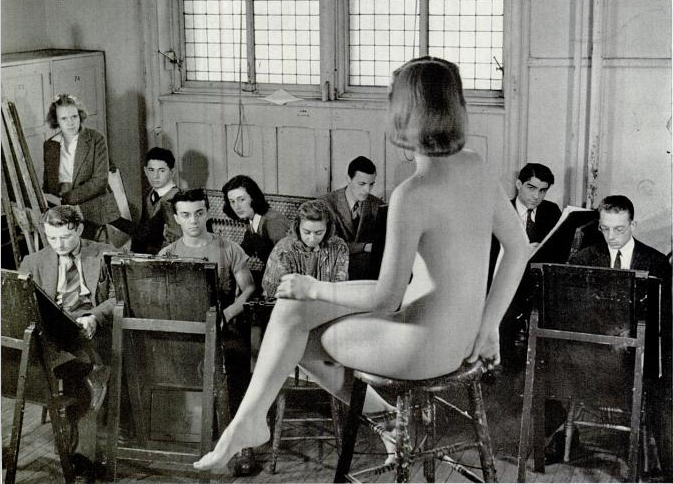
\includegraphics[scale=0.85]{./images/yaleartschool.png}
  \end{sidewaysfigure}

\subsection{Coding for landscape tables}

A landscape table is illustrated in Table~\ref{warefeatures}. Note that you must add the label information twice (in this case, \verb"warefeatures"). Also, you only need to use the minipage environment \verb"\begin{minipage}...\end{minipage}" if your table contains a footnote. Here is the source code:
\begin{smallverbatim}
  \begin{sidewaystable}{warefeatures}
    \caption[Landscape table]{Grooved ware and beaker features,
      their finds and radiocarbon dates. For a breakdown of the
      pottery assemblages see Tables~I and~III; for the flints see
      Tables~II and~IV; for the animal bones see Table~V.}
    \label{warefeatures}
    \begin{minipage}{440pt}% use only if you have a table footnote
    %\smallertablesize % uncomment if your table does not fit the depth
    \begin{tabular}{@{}lcccllccc@{}}
    \hline\hline
    Context\footnote{If you are using footnotes, you must be in a minipage
      environment.}
    & Length & Breadth/ & Depth & Profile & Pottery & Flint
    & Animal & C14 Dates\\
    & & Diameter & & & & & Bones\\[5.5pt]
    & m & m & m\\
    \hline\\[-5.5pt]
    \multicolumn{9}{@{}l}{\textbf{Grooved Ware}}\\
    784 & -- & 0.9$\phantom{0}$ &0.18  & Sloping U & P1     & $\times$46
        & $\phantom{0}$$\times$8  & 2150 $\pm$100\,\textsc{bc}\\
    785 & -- & 1.00             &0.12  & Sloping U & P2--4  & $\times$23
        & $\times$21 & --\\
    962 & -- & 1.37             &0.20  & Sloping U & P5--6  & $\times$48
        & $\times$57 &  1990 $\pm$80\,\textsc{bc} (Layer 4)\\
    & & & & & & & & 1870 $\pm$90\,\textsc{bc} (Layer 1)\\
    983 & 0.83     & 0.73       &0.25  & Stepped U & --     & $\times$18
    & $\phantom{0}$$\times$8  & --\\[\baselineskip]
    \multicolumn{9}{@{}l}{\textbf{Beaker}}\\
    552 & -- & 0.68             & 0.12 & Saucer    & P7--14 & --
        &-- &--\\
    790 & -- & 0.60             & 0.25 & U         & P15    & $\times$12
        & --   &--\\
    794 & 2.89                  & 0.75 & 0.25      & Irreg. & P16
        & $\phantom{0}$$\times$3  &-- &--\\
    \hline\hline
    \end{tabular}
    \end{minipage}
  \end{sidewaystable}
\end{smallverbatim}

% Sideways table
  \begin{sidewaystable}%{warefeatures}
   \captionsetup{type=table, justification=raggedright, width=6cm,margin=0cm, textfont=small}
    \caption[Landscape table]{Grooved ware and beaker features,
      their finds and radiocarbon dates.\\ For a breakdown of the
      pottery assemblages\\ see Tables~I and~III; for the flints see
      Tables~II and~IV; for the animal bones see Table~V.}
      
    \label{warefeatures}
    \begin{minipage}{440pt}% use only if you have a table footnote
    %\smallertablesize % uncomment if your table does not fit the depth
    \begin{tabular}{@{}lcccllccc@{}}
    \hline\hline
    Context\footnote{If you are using footnotes, you must be in a minipage
      environment.}
    & Length & Breadth/ & Depth & Profile & Pottery & Flint
    & Animal & C14 Dates\\
    & & Diameter & & & & & Bones\\[5.5pt]
    & m & m & m\\
    \hline\\[-5.5pt]
    \multicolumn{9}{@{}l}{\textbf{Grooved Ware}}\\
    784 & -- & 0.9$\phantom{0}$ &0.18  & Sloping U & P1     & $\times$46
        & $\phantom{0}$$\times$8  & 2150 $\pm$100\,\textsc{bc}\\
    785 & -- & 1.00             &0.12  & Sloping U & P2--4  & $\times$23
        & $\times$21 & --\\
    962 & -- & 1.37             &0.20  & Sloping U & P5--6  & $\times$48
        & $\times$57 &  1990 $\pm$80\,\textsc{bc} (Layer 4)\\
    & & & & & & & & 1870 $\pm$90\,\textsc{bc} (Layer 1)\\
    983 & 0.83     & 0.73       &0.25  & Stepped U & --     & $\times$18
    & $\phantom{0}$$\times$8  & --\\[\baselineskip]
    \multicolumn{9}{@{}l}{\textbf{Beaker}}\\
    552 & -- & 0.68             & 0.12 & Saucer    & P7--14 & --
        &-- &--\\
    790 & -- & 0.60             & 0.25 & U         & P15    & $\times$12
        & --   &--\\
    794 & 2.89                  & 0.75 & 0.25      & Irreg. & P16
        & $\phantom{0}$$\times$3  &-- &--\\
    \hline\hline
    \end{tabular}
    \end{minipage}
  \end{sidewaystable}

\cxset{author block=false}

\restoregeometry






\makeatother
\section{Basic Description:}
This chapter style has the unique characteristic that the chapter number is spelled out, rather than being in arabic numerals. 


\begin{figure}[ht]
\centering
\fbox{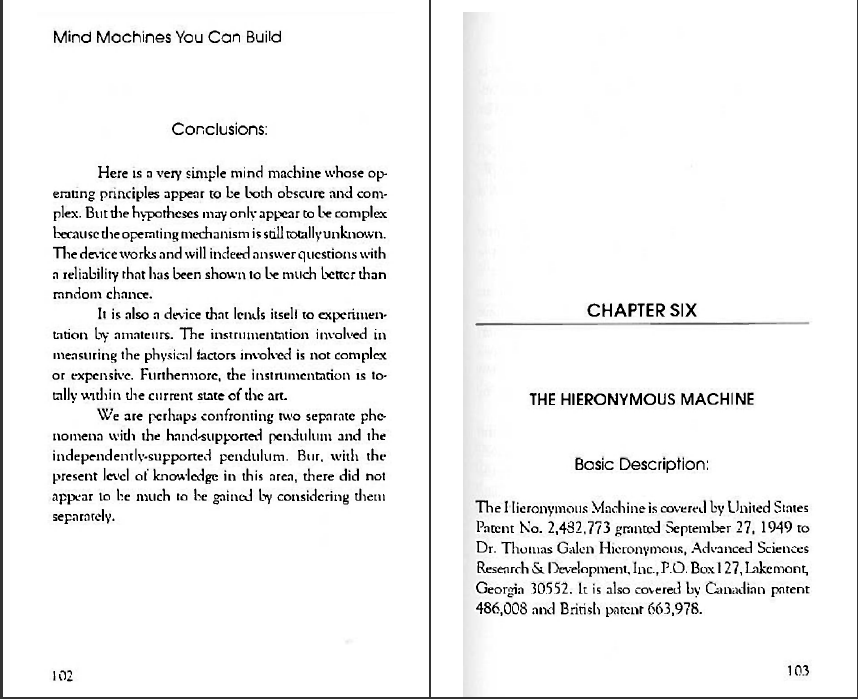
\includegraphics[width=0.6\textwidth]{./chapters/chapter10}}
\caption{Style ten example.}
\end{figure}

Another interesting aspect is that subsection are centered and have a colon at the end of the subsection title. The setting for this is the option \lstinline{numeric=WORDS}. Use either a capital for uppercase or \lstinline{numeric=words} for lowercase number labels.
\end{document}

